\chapter{Recurrent Neural Networks for Semantic Segmentation}\label{sec:reseg}

\autoref{sec:renet} introduced the ReNet model, an RNN-based model for object
recognition. The ReNet model scans the image horizontally and vertically with
$4$ RNNs at each layer and is able to capture the full context of the input
with just one layer thanks to a sophisticated interaction of the inner RNNs.
This allows activations to be local yet conditioned on global information, an
ideal setting for semantic segmentation.

% Intro to semantic segmentation
\emph{Semantic segmentation} is the task of labeling each pixel of an image
with the class it belongs to. In an urban scene scenario, this would mean,
e.g., to label all the pixels of all the cars in the image as belonging to the
"car class", every pixel of all the pedestrians in the image as belonging to
the pedestrian class, and so on.

This is a very difficult task for many reasons: classifying pixels requires to
acquire both a global understanding of the scene, as well as a very detailed
and spatially precise characterization of each object; drawing segmentation
masks is very time consuming, which makes it difficult and expensive to collect
big datasets; labels are often subject to personal judgement, in fact different
people tend to have different degrees of accuracy on small details and
contours and at the same time, it is hard to define a clear separation path
between the object and the background sometimes (e.g., the leafs of a tree)

Segmentation is of paramount importance in many fields that range from
autonomous driving -- where the objects in the scene have to be correctly and
precisely detected to allow the navigation in the environment -- to medical
applications such as magnetic resonance (MR) images analysis, ultrasonography,
surgery robots control or polyps detection in colonoscopies.

% Kinds of semantic segmentation problems
Semantic segmentation is a broad area of research that encompasses many
subtasks, which depend on the kind of images at hand as well as on the domain
of application. The input is usually an image that can be in grayscale or
colors.  In some cases it is required to segment a single image, while
sometimes the task is simplified by the presence of stereo images pairs that
allow to exploit the disparity information, i.e., the difference between the
two images due to the displacement of the cameras. This extra information can
be used to compute a (usually noisy) depth map that can be very helpful to
distinguish between objects that are overlapping in the 2D image, but can be
easily separated on the depth axis. Similarly, depth sensors that produce RGB-D
data can be used in this fashion to improve the segmentation in some domains.
An analogous but slightly different case is that of sparse 3D data, where the
depth information of some points is provided but the measurements are not
densely placed in the input space.
Finally, a related yet distinct setting is the one of cosegmentation, where
multiple images of the same scene have to be segmented. Ideally one would want
the segmentation masks to be consistent across different images. This extra
constraint can be used as a prior to improve those parts that are difficult to
segment in one image but trivial in another.

% How tackled historically
Historically the computer vision community has tackled this problem by building
very specialized hand-engineered algorithms that relied heavily on very
specific domain knowledge. Many of these methods addressed the segmentation
problem looking for highly discriminative local and global features, such as
pixel color (possibly in multiple color spaces, see e.g.,~\citep{
cheng2001color}); histogram of oriented gradients (HoG)~\citep{Dalal05,
bourdev2010detecting,felzenszwalb2010object} -- where the input space is
described with a discrete function that maps locations to colors and the
gradient on the two axes is used to produce a histogram representation of each
patch -- or the similar bag of visual words (BOV)~\citep{csurka2004visual}; the
many local patch descriptors such as SIFT~\citep{lowe2004distinctive},
SURF~\citep{bay2008speeded}, Kaze~\citep{alcantarilla2012kaze}, CenSurE~\citep{
agrawal2008censure}, BRISK~\citep{leutenegger2011brisk}; poselets~\citep{
brox2011object,bourdev2010detecting}, that annotate keypoints of the object to
be detected; dimensionality reduction methods (see e.g., principal components
analysis (PCA)~\citep{smith2002tutorial,shlens2014tutorial,chen2011pixel} and
ZCA whitening~(see e.g.,~\citep{KrizhevskyHinton2009} for a good
introduction)).

Other classical methods for semantic segmentation include clustering
algorithms~\citep[see e.g.,~][]{hartigan1975clustering,chen1998image}, that
group pixel in clusters based on some metrics; graph-based
methods that build a graph with pixels as nodes and some measure of
dissimilarity as weight for the edges~\citep[see e.g.,~][]{
carreira2010constrained,felzenszwalb2004efficient}; active contour models
(ACMs) that segment the image roughly along edges and minimize an energy
function that imposes a smoothness prior on the segmentation~\citep[see
e.g.,~][]{atkins1998fully,kass1988snakes}; watershed segmentation, that takes
the intensity values of grayscale images as a height map and imagines to drop
water on it, filling regions with similar heights until the rise of the water
connects two basins and a watershed is found~\citep[see e.g.,~][]{
roerdink2000watershed}. Finally, many segmentation strategies base on two very
well known and studied algorithms in the literature, namely random decision
forests~\citep{ho1995random,shotton2008semantic} and support vector machines
(SVMs)~\citep{burges1998tutorial,yang2012layered}.

Many of these methods rely on a sliding-window approach, i.e., a classifier
that segments a window of fixed size that moves across the image processing it
in every location. The downside of this approach is that the classification is
performed locally and the full context is usually not captured easily.

The typical strategy to contrast this lack of high level consistency is to pair
the segmentation algorithm with a Markov Random Field (MRF)~\citep[see
e.g.,~][]{ blake2011markov,MurphyBook2012,moser2012markov} or a Conditional
Random Field (CRF)~\citep[see e.g.,~][]{russell2009associative,
he2004multiscale, shotton2006textonboost}. These methods can be implemented in
several ways, but usually impose a local prior on each location and consistency
constraints on pairs or sets of positions. The underlying intuition of these
methods is that the prediction in every location should be consistent with the
one of the neighbouring locations. The pattern of these dependencies can vary
across different implementations and is usually defined based on specific
domain knowledge. For a complete survey on segmentation,
see~\citep{thoma2016survey}.

This chapter introduces the second main contribution of this work. The ReSeg
model~\citep{Visin_2016_CVPR_Workshops} builds on
ReNet~(see~\autoref{sec:renet}) to tackle the task of semantic segmentation.
The primary motivation behind ReSeg is to exploit the peculiar structure of
ReNet in order to capture the underlying semantic of the input image and use it
to drive the prediction in each location, i.e., pixel. Thanks to the strong
lateral connections built in the model, ReSeg is able to capture the
\emph{global} scene depicted in the image and exploit it to perform fine, high
resolution, semantic segmentation focusing on \emph{local} details.

This work extends the preliminary results of~\citep{visin2015renet} modifying
and extending the ReNet model to the more ambitious task of object
segmentation. The performance of the proposed model are tested on some of the
historically most used datasets in this field, namely the Weizmann~Horse
dataset~\citep{Borenstein04combiningtop-down}, the Oxford~Flowers~17
dataset~\citep{Nilsback06} and the more recent and challenging Camvid
dataset~\citep{Brostow2010semantic,BrostowECCV08}. The first two are
tackled in a foreground/background segmentation setting as a proof of concept
for the proposed ReSeg architecture. The performance of the model is then
tested on the full segmentation task on Camvid, a standard benchmark of urban
scenes.

The experiments show that the proposed adaptation of the ReNet for pixel-level
object segmentation performs successfully on the object segmentation task
achieving state-of-the-art performance in all three datasets and may have
further applications in other structured prediction problems.\footnote{
    Subsequent but independent work~\citep{DBLP:journals/corr/YanZJBY16}
    further confirmed the effectiveness of ReSeg, combining a variation of it
    with CRFs and reporting state of the art results on Pascal
    VOC~\citep{Everingham15}.}
Furthermore, the ReNet and ReSeg architectures could be easily merged into a
joint network to perform both tasks at the same time, sharing most of the
computation. This could be interesting in application domains where object
classification and segmentation have to be performed simultaneously,
e.g., autonomous driving and object retrieval.

In the following of the chapter, \autoref{sec:reseg_rationale} motivates the
model in the context of the state of the art at the time it was conceived,
\autoref{sec:reseg_model} describe the ReSeg model in detail and
\autoref{sec:reseg_experiments} presents the results of the experiments.


\section{Motivation}\label{sec:reseg_rationale}

In recent years, CNNs have become the {\em de facto} standard in many computer
vision tasks, such as image classification and object detection
\citep{Krizhevsky-2012,Erhan2014}. Top performing image classification
architectures usually involve {\em very} deep CNN trained in a supervised
fashion on large datasets~\citep{Lin2014,Simonyan2015, szegedy2014going} and
have been shown to produce generic hierarchical visual representations that
perform well on a wide variety of vision tasks.

Similarly, in the semantic segmentation panorama there is a tendency to convert
the standard deep CNN classifier into Fully Convolutional Networks (FCN) (see
e.g.,~\citep{long2014fully,noh2015learning, badrinarayanan2015segnet,
Ronneberger2015}) to obtain coarse image representations, which are
subsequently upsampled to recover the lost resolution. However, these deep CNNs
heavily reduce the input resolution through successive applications of pooling
or subsampling layers. While these layers seem to contribute significantly to
the desirable invariance properties of deep CNNs, they also make it challenging
to use these pre-trained CNNs for tasks such as semantic segmentation, where a
per pixel prediction is required.

%% Upsampling
The problem of recovering pixel level information from the inner layers of a
CNN has been tackled in a large variety of ways. For instance,
\citep{eigen2015predicting} proposed a multi-scale architecture that extracts
coarse predictions, which are then refined using finer scales.
\cite{Farabet:2013} introduced a multi-scale CNN architecture;
\cite{Hariharan2015} combine the information distributed over all layers to
make accurate predictions. Other methods such
as~\citep{long2014fully,badrinarayanan2015segnet} use simple bilinear
interpolation to upsample the feature maps of increasingly abstract layers and
\cite{Ronneberger2015} concatenate the feature maps of the downsampling layers
with the feature maps of the upsampling layers to help recover finer
information. Finally, more sophisticated upsampling methods, such as
unpooling~\citep{noh2015learning,badrinarayanan2015segnet} or
deconvolution~\citep{long2014fully} are now well established in the literature.

One common issue of all these methods is that they are not specifically
designed to take into account and preserve both \emph{local} and \emph{global}
contextual dependencies, which have shown to be useful for semantic
segmentation tasks~\citep{Singh2013,Gatta14-deepvision}. Rather, these models
often employ Conditional Random Fields (CRFs) as a post-processing step to
locally smooth the model predictions, but how to tackle long-range contextual
dependencies remains relatively unexplored.

%% What we propose
Recurrent neural networks have been used in a variety of tasks for years and
have been particularly successful in natural language processing~\citep[see,
e.g.,][]{Mikolov-thesis-2012,Sutskever-et-al-NIPS2014,Cho2014}, handwriting
recognition and generation~\citep[see, e.g.,][]{Graves+Schmidhuber-2009,
Graves-et-al-NIPS2007,Graves-arxiv2013} and speech recognition~\citep[see,
e.g.,][]{Chorowski-et-al-arxiv2014,Graves+Jaitly-ICML2014}. Only recently RNN
and RNN-like models have become popular in the semantic segmentation literature
to capture long distance pixel dependencies with the goal to improve semantic
segmentation~\citep{Pinheiro:2014,Gatta14-deepvision,chen2015semantic,
byeon2015scene,stollenga2015parallel}.

For instance, in~\citep{Pinheiro:2014,Gatta14-deepvision}, CNN are
unrolled through different time steps to include semantic feedback connections.
In~\citep{byeon2015scene}, 2-dimensional Long Short Term Memory, which
consist of 4 LSTM blocks scanning all directions of an image (left-bottom,
left-top, right-top, right-bottom), are introduced to learn long range spatial
dependencies. Following a similar direction, in~\citep{stollenga2015parallel},
multi-dimensional LSTM are swept along different image directions; however, in
this case, computations are re-arranged in a pyramidal fashion for efficiency
reasons. Finally, in~\citep{visin2015renet}, ReNet is proposed to model pixel
dependencies in the context of image classification. It is worth noting that
an important consequence of the adoption of the ReNet spatial sequences is
that they are even more easily parallelizable, as each RNN is dependent only
along a horizontal or vertical sequence of pixels; i.e., all rows/columns of
pixels can be processed at the same time.

The ReSeg model, that is the subject of this chapter, aims to be an {\em
efficient} application of recurrent Neural networks to retrieve contextual
information from images. The goal of this model is to extend the ReNet
architecture~\citep{visin2015renet}, originally designed for image
classification, to deal with the more ambitious task of semantic segmentation.

As explained in~\autoref{sec:renet} the ReNet layers can efficiently
capture contextual dependencies from images by first sweeping the image
horizontally, and then sweeping vertically the feature maps produced by the
horizontal processing. The output of a ReNet layer is therefore implicitly
encoding the local features at each pixel position with respect to the whole
input image, providing a rich feature map of local features conditioned on
global information. The intuition behind the proposed ReSeg model is that this
can be exploited for more fine detailed tasks than the object recognition
originally proposed in ReNet, such as to address the pixel-level task of
semantic segmentation.

To decrease the training time and benefit from generic local features, the
ReSeg model first preprocesses the input with a FCN, i.e., the intermediate
convolutional output of VGG-16~\citep{Simonyan2015} is given as an input to the
recurrent part of the network. Multiple ReNet layers then work on this generic
feature map to extract meaningful local and global pixel dependencies.
% Each ReNet layer is composed of four RNN that sweep the image
% horizontally and vertically in both directions, encoding patches or
% activations, and providing relevant global information.
The resulting structured prediction architecture exploits the local generic
features extracted by the CNNs and the ability of RNNs to retrieve distant
dependencies to produce a rich encoding of the input. Finally, one or more
transposed convolutional layer are stacked on top of the ReNet layers to
upsample the intermediate feature maps back to the image size, in order to
allow predictions at the pixel level.

The ReSeg architecture is efficient, flexible and suitable for a variety of
pixel-level, fine grained tasks, e.g., detecting road signs, cars and
pedestrians in autonomous navigation settings; detecting tumors in fMRI scans
or surgical videos; guide autonomous surgical robots by detecting medical
instruments in operations; detect faces and other parts of the human body for
end users applications such as interactive games or camera autofocus.
%The model is evaluated on the semantic segmentation tasks on several
%widely-used datasets: Weizmann~Horse, Oxford~Flower, and CamVid; achieving
%state-of-the-art performance in all of them.
%Results show that ReSeg can act as a suitable architecture for semantic
%segmentation tasks,
The ReSeg source code and model hyperparameters are available on
\href{https://github.com/fvisin/reseg}{https://github.com/fvisin/reseg}.


\section{Model Description}\label{sec:reseg_model}

ReSeg builds on top of ReNet, described in \autoref{sec:renet} and
extends it to address the task of semantic segmentation. The model pipeline
involves multiple stages. First, the input image is processed with the
VGG-16~\citep{Simonyan2015} network, pre-trained on
ImageNet~\citep{imagenet_cvpr09} without further fine-tuning. By design, only
the first layers of VGG-16 have been used to prevent the resolution of the
intermediate feature maps to become too small.  The result of this
preprocessing is then fed into one or more \emph{ReNet layers} that sweep over
the image horizontally and vertically. Finally, one or more \emph{upsampling
layers} are employed to resize the last feature maps to the same resolution as
the input and a softmax non-linearity is applied to predict the probability
distribution over the classes for each pixel. The following sections analyze in
detail each component of the processing pipeline.

\subsection{ReNet layer}

As in the ReNet model, each recurrent layer is composed by 4 RNNs coupled
together in such a way to capture the local and global spatial structure of the
input data. Specifically, the model takes as an input an image (or the feature
map of the previous layer) $\mathbf{X}$ of elements $x \in \RR^{H \times W
\times C}$, where $H$, $W$ and $C$ are respectively the height, width and
number of channels (or features) and splits it into $I \times J$ flattened
non-overlapping patches $\mathbf{p}_{i,j} \in \RR^{H_p \times W_p \times C}$.
It then sweeps along each of its columns $\mathbf{p}_{i,\cdot}$ vertically a
first time with two RNNs $f^{\downarrow}$ and $f^{\uparrow}$, with $U$
recurrent units each, that move top-down and bottom-up respectively. Note that
the processing of each column is independent and can be done in parallel. This
is a very important performance difference of the ReSeg model with respect to
other architectures in the literature that enforce to handle the data in a more
constrainedly sequential nature.

\begin{figure}[t]
    \advance\leftskip-0.2\textwidth
    \centering
    \makebox[\textwidth][c]{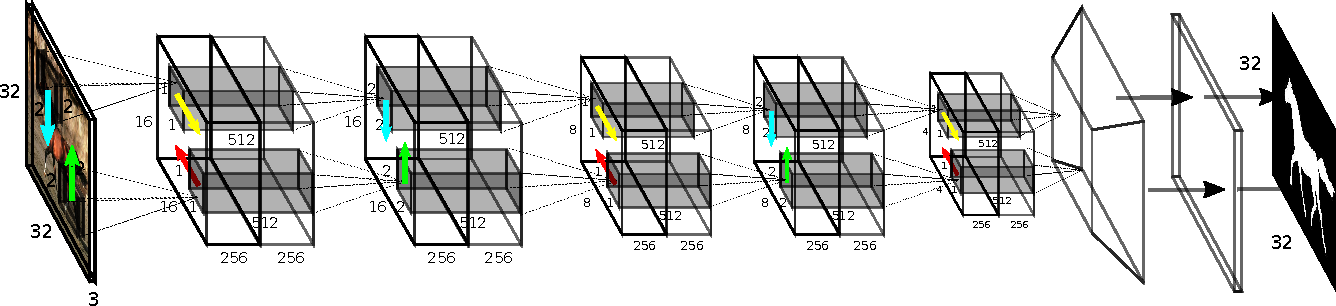
\includegraphics
    	[height=.135\textheight,width=\textwidth]{img/reseg/reseg_base.pdf}}
    \caption{The ReSeg network. For space reasons the pretrained VGG-16
        convolutional and pooling layers used to preprocess the input to ReSeg
        are represented in a compact form in blue and yellow (corresponding to
        the last preprocessed feature map). The first 2 RNNs (blue and green
        arrows) are applied on 2x2x3 patches of the image. Since the patches
        are non-overlapping, this has the effect of halving the resolution. The
        resulting 16x16x256 feature maps are concatenated and fed as input to
        the next two RNNs (red and yellow arrows) which read 1x1x512 patches
        and emit the output of the first ReNet layer. Two similar ReNet layers
        are stacked, followed by an upsampling layer and a softmax
        nonlinearity.}
    \label{fig:ReSeg}
\end{figure}

At every time step each RNN reads the next non-overlapping patch
$\mathbf{p}_{i,j}$ and, based on its previous state, emits a projection
$\mathbf{o}_{i,j}^{\star}$ and updates its state $\mathbf{c}_{i,j}^{\star}$:
\begin{align}
    \mathbf{o}^{\downarrow}_{i,j} =
        f^{\downarrow}(\mathbf{c}^{\downarrow}_{i-1,j},\mathbf{p}_{i,j}),
        &\text{ for }i=1,\cdots, I,\\
    \mathbf{o}^{\uparrow}_{i,j} = f^{\uparrow}(\mathbf{c}^{\uparrow}_{i+1,j},
        \mathbf{p}_{i,j}), &\text{ for }i=I,\cdots,1.
\end{align}
It has to be stressed that the decision to read non-overlapping patches is a
modeling choice to increase the image scan speed and lower the memory usage,
but is not a limitation of the architecture.

Once the first two vertical RNNs have processed the whole input $\mathbf{X}$ in
parallel, their projections $\mathbf{o}^{\downarrow}_{i,j}$ and
$\mathbf{o}^{\uparrow}_{i,j}$ are concatenated to obtain a composite feature
map $\mathbf{O^{\updownarrow}}$ whose elements $\mathbf{o}^{\updownarrow}_{i,j}
\in \RR^{2U}$ can be seen as the activation of a feature detector at the
location $(i,j)$ with respect to all the patches in the $j$-th column of the
input. For simplicity, in the rest of this manuscript this part of the model
will be referred to as \emph{vertical recurrent sublayer}.

After obtaining the concatenated feature map $\mathbf{O^{\updownarrow}}$, the
model sweeps over each of its rows with a pair of new RNNs $f^{\rightarrow}$
and $f^{\leftarrow}$. Each element of $\mathbf{O^{\updownarrow}}$ is processed
individually, rather than grouping them into patches as was done in the
vertical recurrent sublayer. This was chosen so that the second recurrent
sublayer has the same spatial granularity as the first one, but this is not a
constraint of the model and different architectures can be explored.

With a similar procedure as the one adopted for the first sublayer, but in the
horizontal direction, the network reads one element of the intermediate feature
map $\mathbf{o}^\updownarrow_{i,j}$ at each step and emits two activations
coming from two new RNNs that are concatenated into a unique feature map
$\mathbf{O^\leftrightarrow}~=~\left\{ \mathbf{o}^\leftrightarrow_{i,j} \right\}
_{i=1\dots I}^{j=1\dots J}$, with $\mathbf{o}^\leftrightarrow_{i,j} \in
\RR^{2U}$. Each element $\mathbf{o}^\leftrightarrow_{i,j}$ of this
\emph{horizontal recurrent sublayer} represents the features of one of the
input image patches $\mathbf{p}_{i,j}$ \emph{with contextual information from
the whole image}.

It is trivial to note that it is possible to concatenate many recurrent layers
$\mathbf{O^{(1 \cdots L)}}$ one after the other and train them with any
optimization algorithm that performs gradient descent, as the composite model
is a smooth, continuous function.

The recurrent layers that are the core of this architecture, can be either
implemented as vanilla $\tanh$ RNN layers, Gated Recurrent Unit~(GRU)
layers~\citep{Cho2014} or LSTM~layers~\citep{Hochreiter+Schmidhuber-1997}.
Previous work has shown that the ReNet model can perform well with little
concern for the specific recurrent unit used~\citep{visin2015renet}. The ReSeg
model was tested choosing GRU units over alternative implementations, as
they strike a good balance between memory usage and computational power, but
nothing prevents from using different kinds of RNN layers.

\subsection{Upsampling layer}\label{sec:upsampling}

Since by design each recurrent layer processes non-overlapping patches, the
size of the last composite feature map is smaller than the size of the
initial input $\mathbf{X}$, whenever the patch size is greater than one. To be
able to compute a segmentation mask at the same resolution as the ground truth,
the prediction has to be expanded back before applying the softmax
non-linearity.

Several different methods can be used to this end, e.g., fully connected
layers, full convolutions and transposed convolutions. The first is not a good
candidate in this domain as it does not take into account the topology of the
input, which is essential for this task; the second is not optimal either, as
it would require large kernels and stride sizes to upsample by the required
factor. Transposed convolutions are both memory and computation efficient, and
are the ideal method to tackle this problem.

Transposed convolutions~(introduced in \autoref{sec:transposed_conv}) -- also
known as \emph{fractionally strided convolutions} -- have been employed in many
works in recent literature~\citep{Zeiler-ICCV2011,ZeilerFergus14,long2015fully,
radford2015unsupervised,im2016generating}. This method is based on the
observation that direct convolutions can be expressed as a dot product between
the flattened input and a sparse matrix, whose non-zero elements are elements
of the convolutional kernel. The equivalence with the convolution is granted by
the connectivity pattern defined by the matrix.

Transposed convolutions apply the transpose of this transformation matrix to
the input, resulting in an operation whose input and output shapes are inverted
with respect to the original direct convolution. A very efficient
implementation of this operation can be obtained exploiting the gradient
operation of the convolution -- whose optimized implementation can be found in
many of the most popular libraries for neural networks. For an in-depth and
comprehensive analysis of each alternative,
%we refer the interested reader to~\citep{dumoulin2016guide}.
see~\autoref{sec:transposed_conv}.


\section{Experiments}\label{sec:reseg_experiments}

\subsection{Datasets}

The ReSeg architecture has been evaluated on several benchmark datasets. The
model has been first tested on the easier case of background/foreground
segmentation, where the algorithm is only requested to distinguish between the
main subject in the scene and the rest of the image. These preliminary
experiments were conducted on the Weizmann Horse and the Oxford Flowers
datasets, to then focus on the full task of semantic segmentation on the more
challenging Camvid dataset. The rest of this section proceeds as follows: each
dataset is briefly introduced, the settings of each experiment are then
outlined and finally the results are presented and discussed.

\subsubsection{Weizmann Horse}
The Weizmann Horse dataset, introduced in~\citep{Borenstein04combiningtop-down}
\footnote{http://www.msri.org/people/members/eranb/},
is an image segmentation dataset consisting of 329 variable size images in both
RGB and gray scale format, matched with an equal number of groundtruth
segmentation images, of the same size as the corresponding image. The
groundtruth segmentations contain a foreground/background mask of the focused
horse, encoded as a real-value between 0 and 255. To convert this into a
boolean mask, the data has been thresholded in the center of the range setting
all smaller values to 0, and all greater values to 1. See~\autoref{%
fig:reseg_samples_horses} for some segmentation samples.

\begin{figure}[t!]
    \centering
    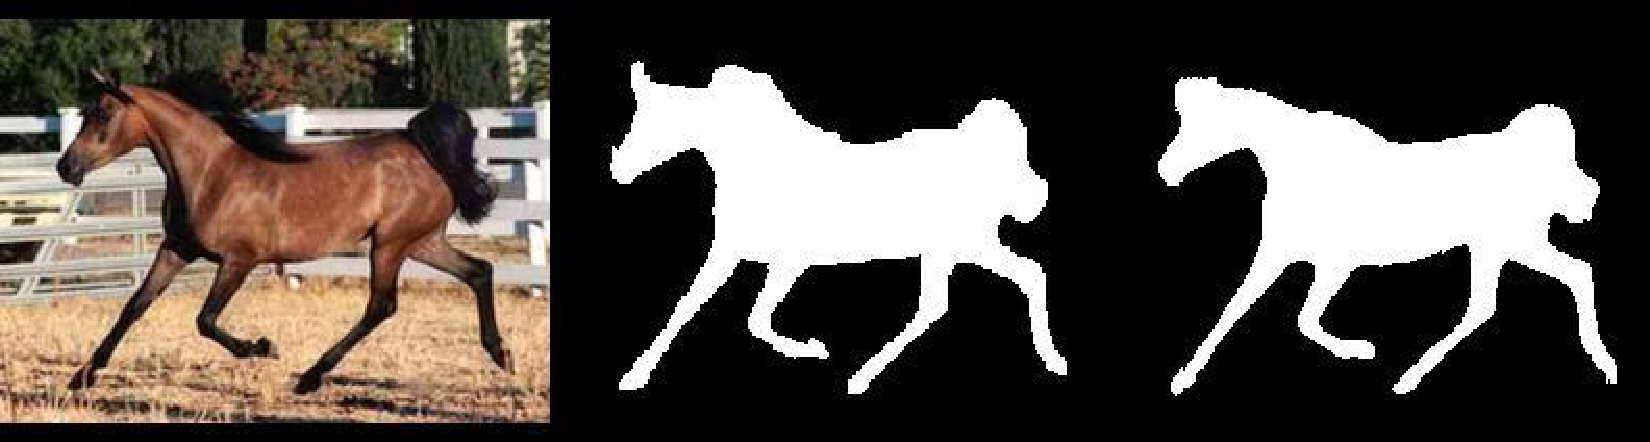
\includegraphics[width=\textwidth]{img/reseg/samples/horse1.pdf}\\
    \vspace{0.1em}
    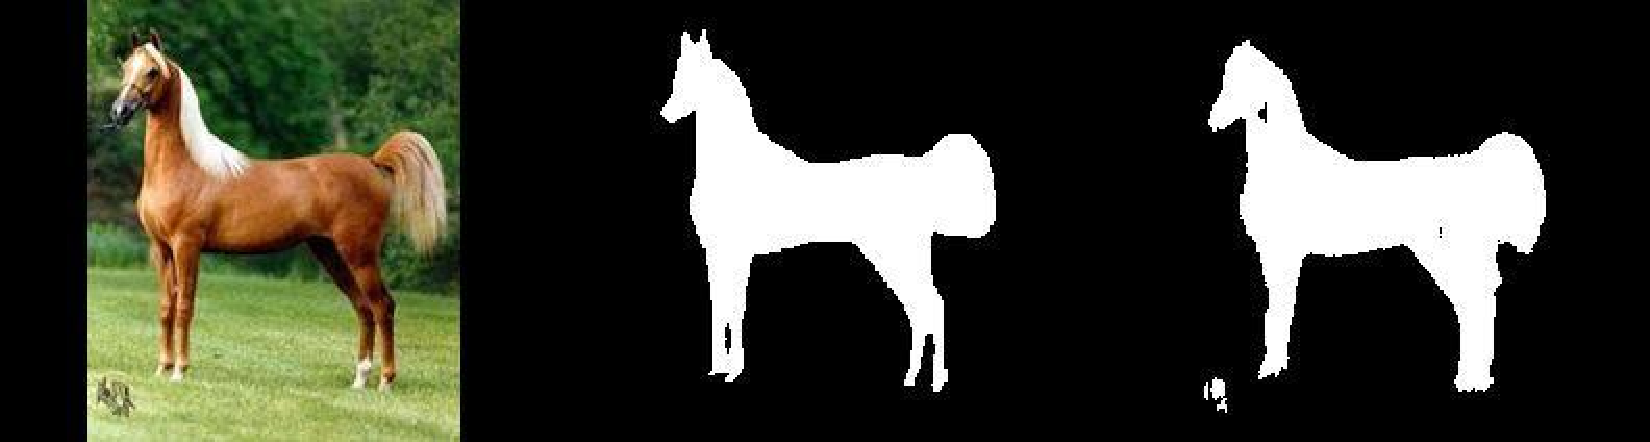
\includegraphics[width=\textwidth]{img/reseg/samples/horse2.pdf}
    \caption{ReSeg Weizmann Horse segmentation samples.
        Left: Input image, Center: Ground truth segmentation,
        Right: ReSeg predicted segmentation.}
    \label{fig:reseg_samples_horses}
\end{figure}

% \subsubsection{Fashionista}
% The Fashionista dataset from ~\citep{Fashionista} contains 685 RGB images of
% fashion models wearing a variety of different clothing.
% Each image and its corresponding mask are 400 pixels in width by 600 pixels
% in height, with encoded values for 53 clothing items. In this work we focus
% on foreground/background segmentation, and build the appropriate
% masks from the more complex maps provided by the dataset by creating a new map
% which preserves the background class as 0, and sets pixels which belong to all
% other classes to 1. This appears to be the same procedure undertaken in
% ~\citep{yang2015patchcut} to create a foreground/background task for this dataset.

\subsubsection{Oxford Flowers 17}
The Oxford Flowers 17 class dataset from~\citep{Nilsback06}\footnote{%
http://www.robots.ox.ac.uk/~vgg/data/flowers/} contains 1363
variable size RGB images, with 848 image segmentations maps associated with
a subset of the RGB images. There are 8 unique segmentation classes defined
over all maps, including flower, sky, and grass. To build a
foreground/background mask, the original segmentation maps have been merged
together setting any pixel not marked as class 38 (the flower class) to 0, and
setting all the flower class pixels to 1. This binary segmentation task for
Oxford Flowers 17 is described in detail in~\citep{Xiaomeng14}.
%A larger 102 class Oxford Flowers dataset is available from the same authors.
See~\autoref{fig:reseg_samples_flowers} for some segmentation samples.

\begin{figure}[t!]
    \centering
    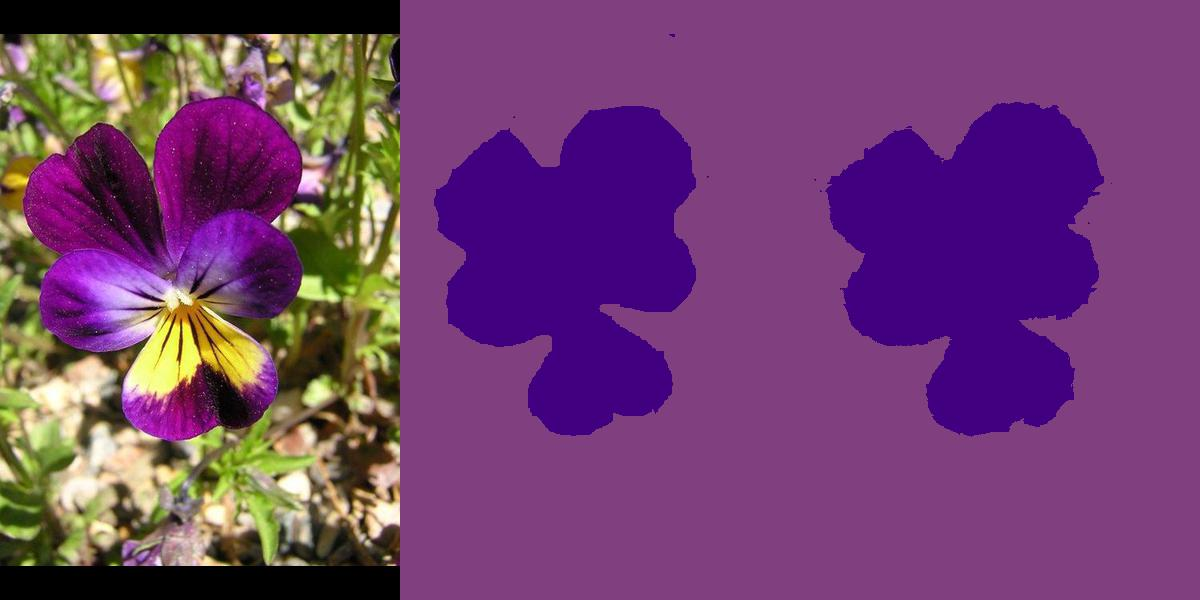
\includegraphics[width=0.5\textwidth]{img/reseg/samples/flowers1.jpg}\\
    \vspace{0.1em}
    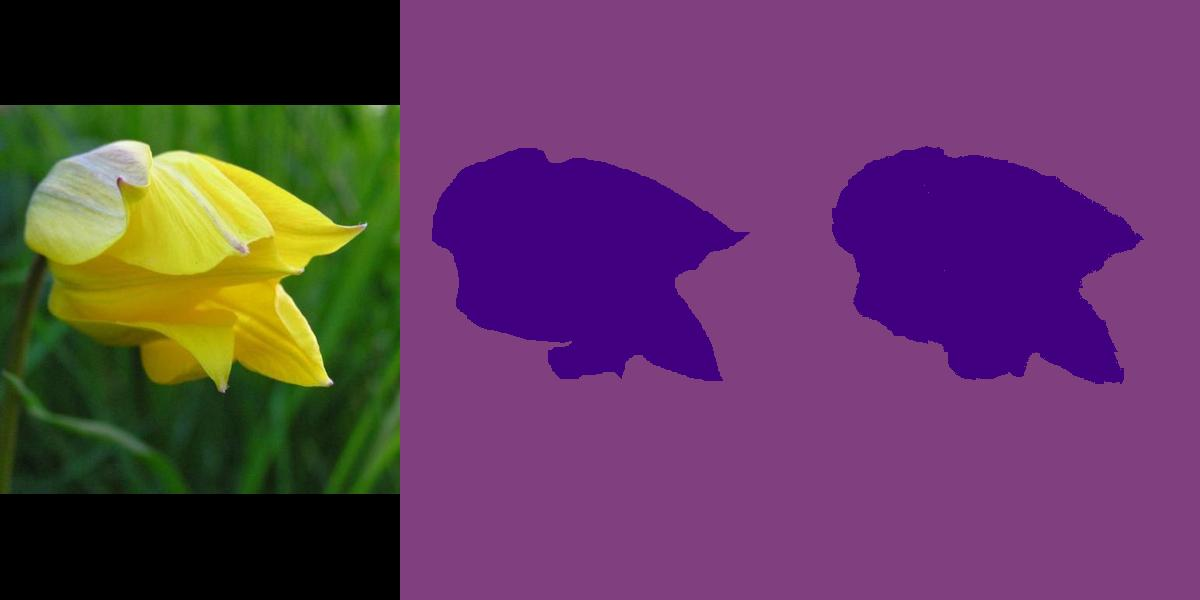
\includegraphics[width=0.5\textwidth]{img/reseg/samples/flowers2.jpg}
    \caption{ReSeg Oxford Flowers segmentation samples.
        Left: Input image, Center: Ground truth segmentation,
        Right: ReSeg predicted segmentation.}
    \label{fig:reseg_samples_flowers}
\end{figure}

\subsubsection{CamVid Dataset}\label{sec:reseg+camvid}
The Cambridge-driving Labeled Video Database (CamVid)~\citep{
Brostow2010semantic}~\footnote{%
http://mi.eng.cam.ac.uk/research/projects/VideoRec/CamVid/}
is a real-world dataset which consists of images recorded from a car with an
internally mounted camera, capturing frames of $960 \times 720$ RGB pixels per
frame, with a recording frame rate of 30 frames per second.  A total of ten
minutes of video was recorded, and approximately one frame per second has been
manually annotated with per pixel class labels, from one of 32 possible
classes. A small number of pixels were labeled as void in the original
dataset. These do not belong to any of the 32 classes prescribed in the
original data, and are ignored during evaluation. The CamVid dataset is split
into 367 training, 101 validation and 233 test images for a total of 701 images
with corresponding annotations. The results presented in this section were
obtained on a preprocessed version of the dataset that downscaled the images to
a resolution of $480 \times 360$ and used a subset of the original labels that
comprises 11 class categories. This experimental setup was chosen to be able to
compare the results of the model to those reported
in~\citep{badrinarayanan2015segnet}. See~\autoref{fig:reseg_samples_camvid} for
some segmentation samples.

\begin{figure}[t!]
    \centering
    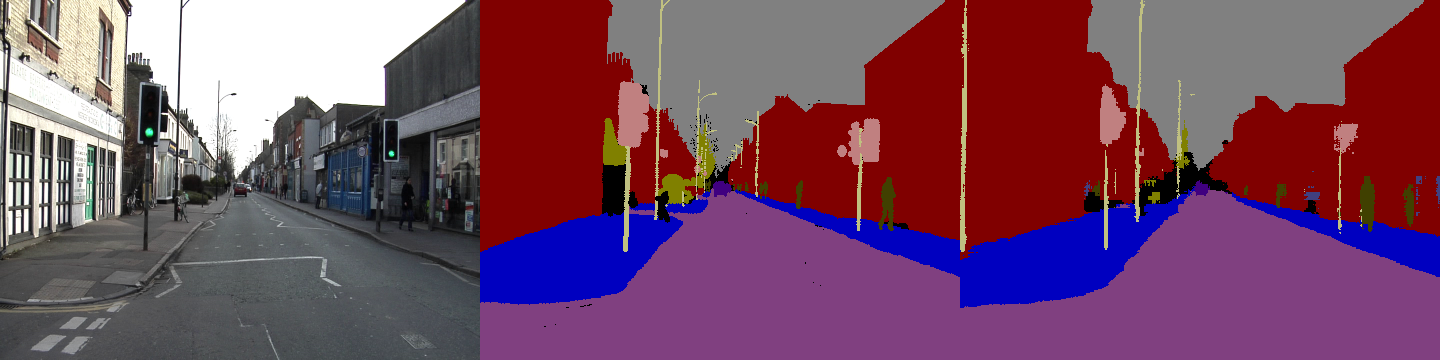
\includegraphics[width=\textwidth]{img/reseg/samples/camvid1.png}\\
    \vspace{0.1em}
    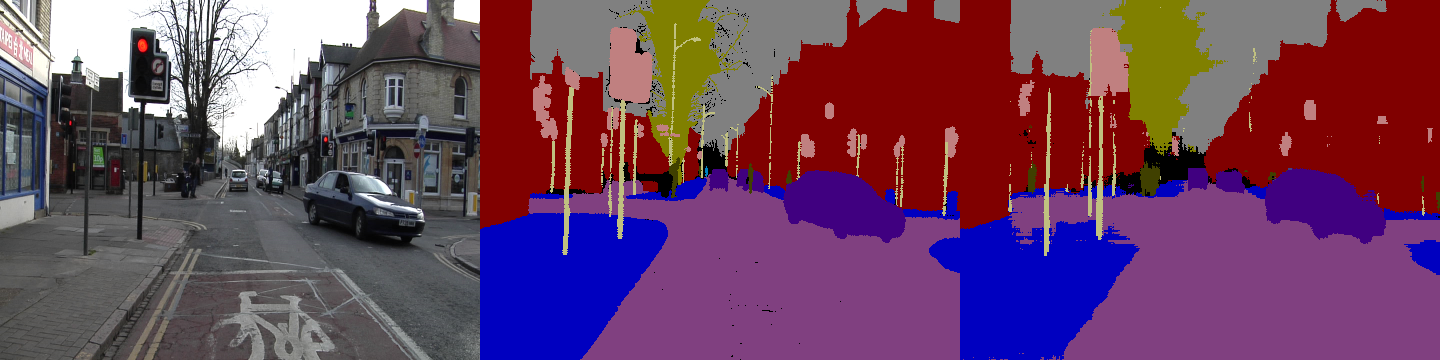
\includegraphics[width=\textwidth]{img/reseg/samples/camvid4.png}
    \caption{ReSeg CamVid segmentation samples.
        Left: Input image, Center: Ground truth segmentation,
        Right: ReSeg predicted segmentation.}
    \label{fig:reseg_samples_camvid}
\end{figure}

\subsection{Data augmentation and preprocessing}\label{sec:data_preprocessing}

The ReNet model adopted some data augmentation methods to enlarge the dataset
by adding synthetic data obtained by randomly flipping and shifting the images.
In ReSeg instead, this kinds of data augmentation were not employed.

The only data augmentation technique exploited was to randomly change the
colors by inverting the intensity values of the whole image with probability
0.5. This kind of data augmentation technique is only meaningful when working
with gray-scale images and was employed for the Weizmann Horse dataset only to
improve the segmentation performance on light colored horses. In that dataset
in fact the light-colored horses are much less represented than the dark ones
and the network did not perform very well on the former without data
augmentation. Its introduction allowed to significantly improve the performance
on the Weizmann Horse dataset, probably because the misclassification of the
few light-colored horses impacted severely on the total score due to the very
limited number of images of the dataset. The same technique would probably not
be as effective on bigger and more balanced datasets.

In the \emph{training} phase, all the images have been resized to the average
resolution of the training set, by computing the mean width and height over the
training set in case of images with variable size. To keep the aspect ratio of
the images unmodified, each image has been first resized to match the shortest
dimension and then center-padded with zeros on the remaining axis to reach the
desired resolution. It should be noted that all transformations that involve
changes in dimensionality or position must also be applied in the same form to
the segmentation mask, and great care must be taken (especially during
resizing/shifting) not to introduce unexpected errors. It is particularly
important to resize the network prediction to the original size of the ground
truth and not the opposite, not to misrepresent the segmentation accuracy. This
is not a problem for validation and test, as the images are not resized in
those cases.

This resizing strategy was adopted for the Weizmann Horse and Oxford Flowers
dataset, while in the Camvid dataset case no resize was needed, apart from the
one reported in~\autoref{sec:reseg+camvid}. This strategy allowed to train on
batches of multiple images, with the effect of speeding up the training fully
exploiting the parallel computation allowed by GPU-computing. The performance
loss due to the difference in training and validation/test size was negligible,
probably thanks to the adoption of the pretrained VGG-16 layers that can
extract meaningful features from the typical size of the images in the adopted
datasets. On the contrary, training benefitted a little from resizing the
images on some of the datasets, probably because eliminating unnecessary and
easily explained variance can help the model focus on harder characteristics,
which generally leads to better performance on the task at hand.
%especially in the case of segmentation where object scale between images has little
%impact on the class category.

\subsection{Experimental settings}

To gain confidence with the sensitivity of the model to the different
hyperparameters, ReSeg was first evaluated on the Weissman Horse and Oxford
Flowers datasets on a binary foreground/background segmentation task. Once a
good initial setting of the hyperparameters was found, most of the efforts were
spent on the more challenging semantic segmentation task on the CamVid dataset.

The number of hyperparameters of this model is potentially very high, as for
each ReNet layer different implementations are possible (namely vanilla RNN,
GRU or LSTM), each one with its specific parameters. Furthermore, the number of
features, the size of the patches and the initialization scheme have to be
defined for each ReNet layer as well as for each transposed convolutional
layer. To make it feasible to explore the hyperparameter space, some of the
hyperparameters have been fixed by design and the remaining have been
finetuned.
In the rest of this section, the architectural choices for both
sets of parameters will be detailed.

Initial experiments on upsampling showed that transposed convolutional layers
seem to provide a better performance with respect to less sophisticated (not
learned) tiling strategies such as nearest neighbor tiling or bilinear
interpolation when there is enough data to learn the transformation. All the
transposed convolution upsampling layers were followed by a
ReLU~\citep{Krizhevsky2012-alexnet} non-linearity and initialized with the
fan-in plus fan-out initialization scheme described
in~\citep{glorot2010understanding}. The recurrent weight matrices were instead
initialized to be orthonormal, following the procedure defined
in~\citep{Saxe2014}. Finally, the stride of the upsampling transposed
convolutional layers was constrained to be tied to their filter size.

One specificity of the segmentation task is that each training image carries
classification information for all of its pixels. Differently from the image
classification task, small batch sizes already provide the model with a large
amount of information with sufficient variance to learn and generalize well.
The ReSeg model was tested with various values of batch size, going as low as
processing a single image at a time, obtaining comparable results in terms of
performance. Many experiments were performed using a minibatch size of 1. When
computational resources allowed, larger batch sizes were used, e.g., 5, 10,
20, 35, and 50. Larger batch sizes smoothed learning (as expected), and removed
some issues related to spurious occurrences in the datasets such as misaligned
or poorly segmented groundtruth masks. This had a bigger impact on the smaller
datasets than on Camvid, where the batch size was kept fixed to the value of
$5$, as a compromise between training speed and memory usage.

All the experiments, used L2 regularization~\citep{Krogh92asimple} with a
weight decay factor of $0.001$ to avoid instability at the end of training.
Also, all the models were trained with the Adam~\citep{kingma2014adam}
optimization algorithm, that does not require a specific hyperparameter tuning.
The effect of batch normalization in RNNs has been a focus of
attention~\citep{Laurent2015}, but it does not seem yet to provide a
reliable improvement in performance, so it was not adopted.

The adaptive learning rate algorithm known as Adam~\citep{Kingma2014} was a
key ingredient to stable learning, though others such as
Adadelta~\citep{Zeiler-2012} were useful during model development. In addition,
gradient norm rescaling was also utilized to help with the problems described
in~\citep{bengio2013advances}. Regularization proved to be another important
part of the process on the smaller Weizmann Horse and Oxford flowers datasets.
For those two, weight noise, as described in~\citep{Graves2011}, with a scale
of 0.075 was applied to all weight matrices before each forward pass in all the
experiments. Dropout~\citep{Srivastava14} on each forward connection with drop
probability of $0.2$ on the input, and/or with drop probability of $0.5$ on the
hidden projections was applied too.

The experiments mainly focused on varying the number of ReNet layers and the
number of upsampling transposed convolutional layers, as well as tuning their
respective parameters, such as the number of features $d_{\text{RE}}(l)$ and
$d_{\text{UP}}(l)$ respectively, and the size of the input patches (or
equivalently of the filters) ${ps}_{\text{RE}}(l)$ and ${fs}_{\text{UP}}(l)$.
The best parameters are reported in~\autoref{tbl:camvid_params}.

% CAMVID RESULTS
\begin{table}[t]
	\resizebox{\textwidth}{!}{%
		\small{%
            \begin{tabular}{c|c|c|c|c|c|c|c|c|c|c|c||c|c|c}

                \multicolumn{1}{c}{Method} & \multicolumn{1}{c}{\rotatebox{90}{Building}} & \multicolumn{1}{c}{\rotatebox{90}{Tree}} & \multicolumn{1}{c}{\rotatebox{90}{Sky}} & \multicolumn{1}{c}{\rotatebox{90}{Car}} & \multicolumn{1}{c}{\rotatebox{90}{Sign-Symbol}} & \multicolumn{1}{c}{\rotatebox{90}{Road}} & \multicolumn{1}{c}{\rotatebox{90}{Pedestrian}} & \multicolumn{1}{c}{\rotatebox{90}{Fence}} & \multicolumn{1}{c}{\rotatebox{90}{Column-Pole}} & \multicolumn{1}{c}{\rotatebox{90}{Side-walk}} & \multicolumn{1}{c}{\rotatebox{90}{Bicyclist}} & \multicolumn{1}{c}{\rotatebox{90}{Avg class acc}} & \multicolumn{1}{c}{\rotatebox{90}{Global acc}} & \multicolumn{1}{c}{\rotatebox{90}{\textbf{Avg IoU}}}\\ \hline \hline

				\multicolumn{15}{c}{\emph{Segmentation models}} \\ \hline
                Super Parsing   \citep{tighe2013superparsing} & \textbf{87.0} & 67.1 & \textbf{96.9} & 62.7 & 30.1 & 95.9 & 14.7 & 17.9 & 1.7 & 70.0 & 19.4 & 51.2 & 83.3 & n/a \\ \hline
				Boosting+Higher order \citep{sturgess2009combining} & 84.5 & 72.6 & \textbf{97.5} & 72.7 & 34.1 & 95.3 & 34.2 & 45.7 & 8.1 & 77.6 & 28.5 & 59.2 & 83.8 & n/a \\ \hline
				Boosting+Detectors+CRF \citep{ladicky2010and} & 81.5 & 76.6 & 96.2 & 78.7 & 40.2 & 93.9 & 43.0 & 47.6 & 14.3 & 81.5 & 33.9 & 62.5 & 83.8 & n/a \\ \hline

				\multicolumn{15}{c}{\emph{Neural Network based segmentation models}} \\ \hline
				SegNet-Basic (layer-wise training \citep{badrinarayanan2015segnetlayerwise}) & 75.0 & 84.6 & 91.2 & 82.7 & 36.9 & 93.3 & 55.0 & 37.5 & 44.8 & 74.1 & 16.0 & 62.9 & 84.3 & n/a \\ \hline
                SegNet-Basic \citep{badrinarayanan2015segnet} & 80.6 & 72.0 & 93.0 & 78.5 & 21.0 & 94.0 & 62.5 & 31.4 & 36.6 & 74.0 & 42.5 & 62.3 & 82.8 & 46.3 \\ \hline
                SegNet \citep{badrinarayanan2015segnet} & \textbf{88.0 } & \textbf{87.3} & 92.3 & 80.0 & 29.5 & \textbf{97.6} & 57.2 & \textbf{49.4} & 27.8 & 84.8 & 30.7 & 65.9 & 88.6 & 50.2 \\ \hline
                \emph{ReSeg + Class Balance} & 70.6 & 84.6 & 89.6 & 81.1 & \textbf{61.0} & 95.1 & \textbf{80.4} & 35.6 & \textbf{60.6} & \textbf{86.3} & \textbf{60.0} & 73.2 & 83.5 & 53.7 \\ \hline
                \textbf{ReSeg} & 86.8 & 84.7 & 93.0 & \textbf{87.3} & 48.6 & \textbf{98.0} & 63.3 & 20.9 & 35.6 & \textbf{87.3} & 43.5 & 68.1 & 88.7 & \textbf{58.8} \\ \hline

				\multicolumn{15}{c}{\emph{Sub-model averaging}} \\ \hline
                \emph{Bayesian SegNet-Basic} \citep{Kendall2015bayesiansegnet} & 75.1 & 68.8 & 91.4 & 77.7 & 52.0 & 92.5 & 71.5 & 44.9 & 52.9 & 79.1 & 69.6 & 70.5 & 81.6 & 55.8 \\ \hline
                \emph{Bayesian SegNet} \citep{Kendall2015bayesiansegnet} & 80.4 & 85.5 & 90.1 & 86.4 & 67.9 & 93.8 & 73.8 & 64.5 & 50.8 & 91.7 & 54.6 & 76.3 & 86.9 & 63.1 \\ \hline

			\end{tabular}
		}
    }
	\vspace*{0.1cm}
    \caption{%
        CamVid. The table reports the per-class accuracy, the average per-class
        accuracy, the global accuracy and the average intersection over union
        (higher is better). The best values and the values within $1$ point
        from the best are highlighted in bold for each column. For completeness
        the Bayesian Segnet models are reported even if they are not directly
        comparable to the others as they perform a form of model averaging.}
    \label{tbl:camvid_SOTA}
\end{table}

% CAMVID PARAMS
\begin{table}[t]
    \resizebox{\textwidth}{!}{%
        \small{%
            \begin{tabular}{c|c|c|c|c|c|c|c|c|c|c|c|c|c|c|c||c|c|c}
                \multicolumn{1}{c}{Model} & \multicolumn{1}{c}{${ps}_{\text{RE}}$}& \multicolumn{1}{c}{$d_{\text{RE}}$} & \multicolumn{1}{c}{${fs}_{\text{UP}}$}& \multicolumn{1}{c}{$d_{\text{UP}}$} & \multicolumn{1}{c}{\rotatebox{90}{Building}} & \multicolumn{1}{c}{\rotatebox{90}{Tree}} & \multicolumn{1}{c}{\rotatebox{90}{Sky}}  & \multicolumn{1}{c}{\rotatebox{90}{Car}}  & \multicolumn{1}{c}{\rotatebox{90}{Sign-Symbol}} & \multicolumn{1}{c}{\rotatebox{90}{Road}} & \multicolumn{1}{c}{\rotatebox{90}{Pedestrian}} & \multicolumn{1}{c}{\rotatebox{90}{Fence}} & \multicolumn{1}{c}{\rotatebox{90}{Column-Pole}} & \multicolumn{1}{c}{\rotatebox{90}{Side-walk}} & \multicolumn{1}{c}{\rotatebox{90}{Bicyclist}} & \multicolumn{1}{c}{\rotatebox{90}{Avg class acc}} & \multicolumn{1}{c}{\rotatebox{90}{Global acc}} & \multicolumn{1}{c}{\rotatebox{90}{\textbf{Avg IoU}}}\\ \hline \hline

                ReSeg + LCN & $(2 \times 2), (1 \times 1)$ & (100, 100) & $(2 \times 2)$ & (50, 50) & 81.5 & 80.3 & \textbf{94.7} & 78.1 & 42.8 & \textbf{97.4} & 53.5 & 34.3 & 36.8 & 68.9 & 47.9 & 65.1 & 84.8 & 52.6 \\ \hline
                ReSeg + Class Balance & $(2 \times 2), (1 \times 1)$ & (100, 100) & $(2 \times 2)$ & (50, 50) & 70.6 & \textbf{84.6} & 89.6 & 81.1 & \textbf{61.0} & 95.1 & \textbf{80.4} & \textbf{35.6} & \textbf{60.6} & \textbf{86.3} & \textbf{60.0} & 73.2 & 83.5 & 53.7 \\ \hline
                \textbf{ReSeg} & $(2 \times 2), (1 \times 1)$ & (100, 100) & $(2 \times 2)$ & (50, 50) & \textbf{86.8} & \textbf{84.7} & 93.0 & \textbf{87.3} & 48.6 & \textbf{98.0} & 63.3 & 20.9 & 35.6 & \textbf{87.3} & 43.5 & 68.1 & 88.7 & \textbf{58.8} \\ \hline
            \end{tabular}%
        }
    }
    \vspace*{0.1cm}
    \caption{%
        Comparison of the performance of different hyperparameter on CamVid.
    }
    \label{tbl:camvid_params}
\end{table}

% \begin{table}[t]
%     \centering{
%         \small
%         \begin{tabular}{l|c|c|c|c|c|c}
%             Dataset & $b$ & $d_{\text{RE}}$ & $w_p$ & $h_p$ & $a_c$ & upscaling\\
%
%             Weissman horses & 1 & [1100, 1300] & 2 & 2 & tanh & grad \\
%             Fashonista & 1 & [400, 400] & 2 & 2 & tanh & linear \\
%             Oxford Flowers & 5 & [150, 150] & 2 & 2 & tanh & linear \\
%         \end{tabular}
%     }
%     \caption{Hyperparameters.}
%     \label{tbl:hyperparams}
% \end{table}


\subsection{Results}\label{sec:reseg_results}

The metrics reported on all the datasets are the per-pixel accuracy~(\emph{%
Global acc}), computed as the percentage of true positives with respect to the
total number of pixels in the image, as well as the average per-class
Intersection over Union (\emph{Avg IoU}), computed on each class as true
positive divided by the sum of true positives, false positives and false
negatives and then averaged. In the full semantic segmentation setting the
per-class accuracy and the average per-class accuracy (\emph{Avg class acc})
are also reported.

% HORSES
\begin{table}[t]
    \centering{
        \small
        \begin{tabular}{l|c||c}
            Method & Global & \textbf{Avg IoU}\\ \hline

            All foreground baseline & 25.4 & 79.9 \\
            All background baseline & 74.7 & 0.0 \\
            Kernelized structural SVM \citep{bertelli2011kernelized} & 94.6 & 80.1 \\
            ReSeg (no VGG) & 94.9 & 79.9 \\
            CRF learning \citep{liu2015crf} & 95.7 & 84.0 \\
            PatchCut \citep{yang2015patchcut} & 95.8 & 84.0 \\
            \textbf{ReSeg} & 96.8 & \textbf{91.6} \\
        \end{tabular}
    }
    \caption{Weizmann Horses. Per pixel accuracy and average IoU are reported
        (higher is better).}
    \label{tbl:WeizmannHorses_SOTA}
\end{table}

\autoref{tbl:WeizmannHorses_SOTA} reports the results on the Weizmann
Horse dataset. On this dataset, the assumption that processing the input image
with some pre-trained convolutional layers from VGG-16 could ease the learning
was verified. Specifically, the experiments were restricted to only using the
first $7$ convolutional layers from VGG, as the goal was to extract some
low-level generic features only and learn the task-specific high-level features
with the ReNet layers. The results indeed show an increase in terms of average
Intersection over Union (IoU) when these layers are being used, confirming that
the ReNet layers can learn good high-level features from generic convolutional
features detected by a pretrained VGG model.

\begin{figure}[t]
    \centering
    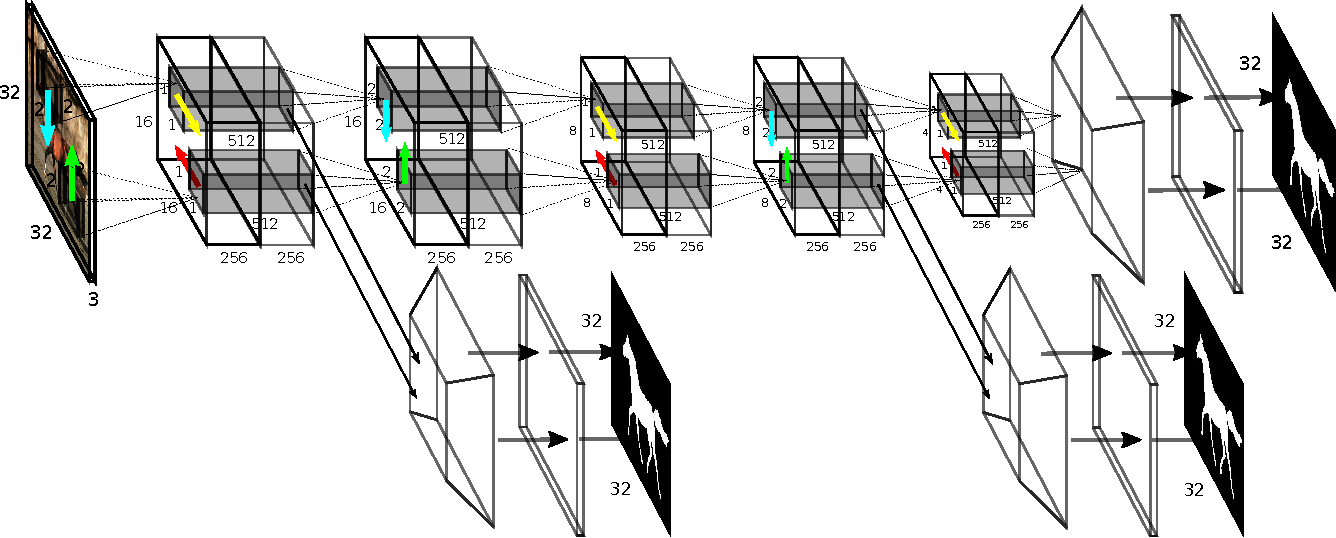
\includegraphics[width=\textwidth]{img/reseg/reseg_interm_pred.pdf}
    \caption{A ReSeg network with intermediate predictions.}
    \label{fig:reseg_intermediate_pred}
\end{figure}

Another variant of the network that was tested on the Weizmann Horse dataset
used intermediate predictions to help the gradient flow in the early layers
of the network as depicted in~\autoref{fig:reseg_intermediate_pred}. In this
scenario, the feature maps of some of the intermediate layers were passed to an
upsampling layer followed by a softmax and the corresponding classification
error was backpropagated to improve the learning of the early layers. The
experiments with this setup were not conclusive, as in some cases the
intermediate layers helped the training while in others they did not seem to
help or were even harmful. Overall, the potential performance improvement was
not significant enough in the positive cases to justify the increase of
complexity and of training time, so it was decided not to employ them in the
following experiments. Recent techniques, such as the use of residual
connections~\citep{he2015deep,srivastava2015training} are most probably more
effective at speeding up the training of early layers of the network.

% FLOWERS
\begin{table}[t]
    \centering{
    \small
        \begin{tabular}{l|c||c}
            Method & Global & \textbf{Avg IoU}\\ \hline

            All background baseline & 71.0 & 0.0 \\
            All foreground baseline & 29.0 & 29.2 \\
            % \textbf{ReSeg (no VGG)} & 86.9 & \textbf{65.8} \\
            GrabCut \citep{rother2004grabcut} & 95.9 & 89.3 \\
            Tri-map \citep{Xiaomeng14} & 96.7 & 91.7 \\
            \textbf{ReSeg} & 98 & \textbf{93.7} \\
        \end{tabular}
    }
    \caption{Oxford Flowers. Per pixel accuracy and average IoU are reported
        (higher is better).}
    \label{tbl:OxfordFlowers_SOTA}
\end{table}

\autoref{tbl:OxfordFlowers_SOTA} shows the results for Oxford Flowers dataset,
when using the full ReSeg architecture (i.e., including VGG convolutional
layers).  As shown in the table, this method clearly outperforms the
state-of-the-art both in terms of global accuracy and average IoU.

Finally, \autoref{tbl:camvid_SOTA} presents the results on CamVid dataset using
the full ReSeg architecture. This model exhibits state-of-the-art performance
in terms of IoU when compared to both standard segmentation methods and neural
network based methods, showing an increase of $17\%$ with respect to the recent
SegNet model. It is worth highlighting that incorporating sub-model averaging
to SegNet model, as in \citep{Kendall2015bayesiansegnet}, boosts the original
model performance, as expected. Therefore, introducing sub-model averaging to
ReSeg could also presumably result in significant performance increase.
However, this remains to be tested.

% There are number of difficulties in directly comparing our performance with the
% reported scores, some of which are intrinsic to using neural based models for
% segmentation, while others are specific to the evaluation datasets or competing
% methodologies.


\section{Discussion}

As pointed out earlier, the experiments on the Weizmann Horse dataset were
treated as a test playground to acquire knowledge on the sensitivity of the
model with respect to the preprocessing and the hyperparameters. The
preliminary experiments show that processing the input images with the first
layers of the VGG-16 pre-trained network improves the results. Other image
manipulation techniques, such as pre-processing the input with Local Contrast
Normalization (LCN), do not seem to improve the performance of the model
(see~\autoref{tbl:camvid_params}) and were therefore not used in the following
experiments.

While the Weizmann Horse and the Oxford Flowers datasets were tackled in a
binary background/foreground segmentation setting, on the CamVid dataset the
full semantic segmentation task was addressed. In this setting, when the
dataset is highly imbalanced, the segmentation performance of some classes can
drop significantly as the network tries to maximize the score on the
high-occurring classes, {\em de facto} \/ignoring the least occurring ones. To
overcome this behaviour, a class-balancing term was added to the cross-entropy
loss to bias the prediction towards the less represented classes. Specifically,
\emph{median frequency balancing}~\citep{eigen2015predicting} was employed,
which re-weights the class predictions by the ratio between the median of the
frequencies of the classes (computed on the training set) and the frequency of
each class:

\begin{equation}
    \alpha(c) = median\_frequency / f(c),
\end{equation}

\noindent where $f(c)$, the frequency of the class $c$, is computed dividing
the number of pixels of the class $c$ by the total number of pixels in the
images \emph{where $c$ is present}, and $median\_frequency$ is the median of
the frequencies of all the classes. The final cross-entropy loss for one image,
rescaled by the rebalancing term is then

\begin{equation}
    cost = -\frac{1}{N} \sum_{i=0}^N \sum_{c=0}^C P(p_i = c) \cdot logQ(p_i= c)
        \cdot \alpha(c),
\end{equation}

\noindent with $N$ the number of pixels in the image, $C$ the number of classes
of the dataset, $P(p_i=c)$ the ground-truth probability of the $i$-th pixel
belonging to the class $c$ and $Q(p_i=c)$ its probability as estimated by the
model. Note that since the ground truth probability of the wrong classes is
usually $0$, the cross-entropy is equivalent to the negative log likelihood of
the correct class under the model's distribution.

Consider the classes ordered by frequency. This rebalancing term assigns a
unitary weight to the central class (i.e., it does not modify its predicted
probability) lower than $1$ to the first half and a weight higher than $1$ to
the second half. The final effect of class balancing is to increase the score
of the low frequency classes (see~\autoref{tbl:camvid_params}) at the price of
a more noisy segmentation mask, as the probability of the underrepresented
classes is overestimated and can lead to an increase in misclassified pixels in
the output segmentation mask. This behavior is clearly visible
in~\autoref{fig:camvid_class_balance}.

\begin{figure}[t]
    \centering
    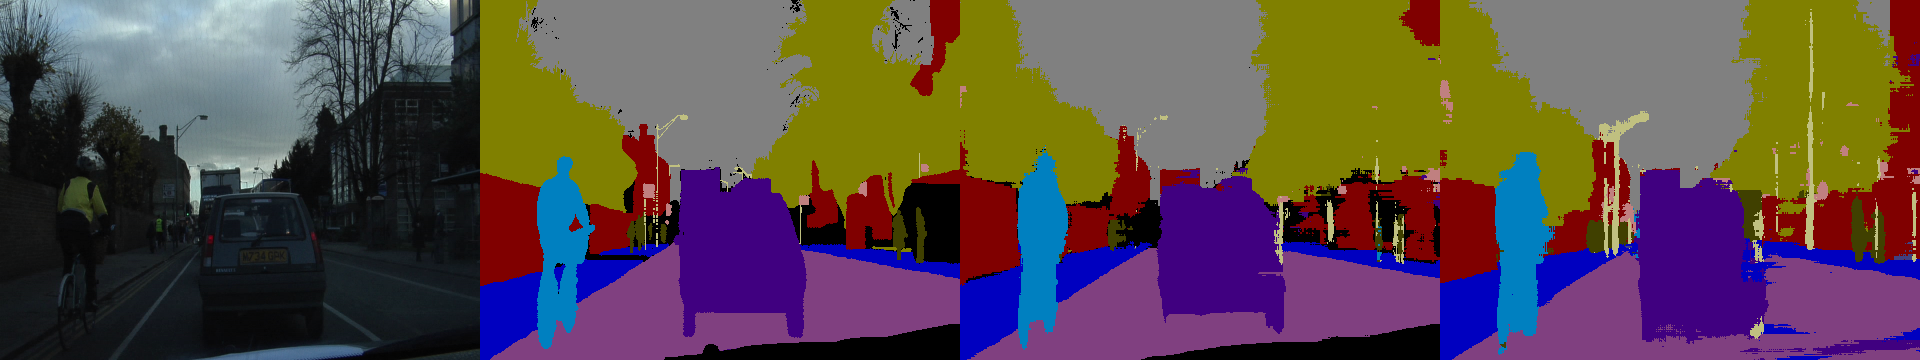
\includegraphics[width=\textwidth]{img/reseg/samples/camvid_classbal_diff.png}
    \caption{Camvid segmentation example with and without class balancing. From
        the left: input image, ground truth segmentation, ReSeg segmentation,
        ReSeg segmentation with class balancing. Class balancing improves the
        low frequency classes, e.g., the street poles, at the price of a
        worse overall segmentation.}
    \label{fig:camvid_class_balance}
\end{figure}

% \section{Conclusion}
% We introduced the ReSeg model, an extension of the ReNet model for image
% semantic segmentation. The proposed architecture shows state-of-the-art
% performances on CamVid, a widely used dataset for urban scene semantic
% segmentation, as well as on the much smaller Oxford Flowers dataset. We also
% report state-of-the-art performances on the Weizmann Horses.
%
% In our analysis, we discuss the effects of applying some layers of VGG-16 to
% process the input data, as well as those of introducing a class balancing
% term in the cross-entropy loss function to help the learning of
% under-represented classes.
Notably, it is sufficient to process the input images with just a few layers of
VGG-16 for the ReSeg model to gracefully handle the semantic segmentation task,
confirming its ability to encode contextual information and long term
dependencies. The dimensionality reduction that derives from halving the
resolution at each encoding layer to expand it back in the upsampling layers
can be expected to cause some loss of spacial precision, especially on
fine-grained details. It is conceivable to imagine that the model could gain
from the introduction of skip connections, a fairly recent technique that
consists in providing higher resolution information from the lower layers to
the upsampling ones. This is described
in~\autoref{sec:deconvLSTM_skip_connections} and adopted in the model that will
be the main subject of the following chapter.

The experiments proved the flexibility of ReSeg in the foreground-background
segmentation as well as the full semantic segmentation tasks on multiple
datasets. The model achieves state of the art on all the datasets it was tested
on and generates convincing segmentation masks, as shown
in~\Autoref{fig:reseg_samples_horses, fig:reseg_samples_flowers,
fig:reseg_samples_camvid, fig:camvid_class_balance}.
